%
% Szakdolgozatminta az Eszterházy Károly Katolikus Egyetem
% matematika illetve informatika szakos hallgatóinak.
%

\documentclass[
% opciók nélkül: egyoldalas nyomtatás, elektronikus verzió
% twoside,     % kétoldalas nyomtatás
% tocnopagenum,% oldalszámozás a tartalomjegyzék után kezdődik
]{thesis-ekf}
\usepackage[T1]{fontenc}
\usepackage{hyperref}
\usepackage{graphicx}
\PassOptionsToPackage{defaults=hu-min}{magyar.ldf}
\usepackage[magyar]{babel}
\usepackage{mathtools,amssymb,amsthm,pdfpages}
\footnotestyle{rule=fourth}

\newtheorem{tetel}{Tétel}[chapter]
\theoremstyle{definition}
\newtheorem{definicio}[tetel]{Definíció}
\theoremstyle{remark}
\newtheorem{megjegyzes}[tetel]{Megjegyzés}

\begin{document}

\institute{Matematikai és Informatikai Intézet}
\title{2D platformer játék fejlesztése unityben}
\author{Bartus János\\Programtervező informatikus}
\supervisor{Troll Ede\\Tanársegéd}
\city{Eger}
\date{2025}
\maketitle

\tableofcontents

\chapter*{Bevezetés}
\addcontentsline{toc}{chapter}{Bevezetés}
Gyerekkorom óta érdekeltek a videójátékok, már egészen kicsiként kezdtem el játszani. Az első komolyabb élményeimet apukám PlayStation 2 konzolján szereztem ahol sok időt töltöttem különböző játékokkal. Akkoriban még csak a játék öröme vonzott, nem is gondoltam volna hogy ennyire mélyen elmerülök ebben a világban.
Ahogy idősebb lettem, általános iskola alsó tagozatában kezdtek jobban érdekelni a videójátékok nemcsak mint szórakozás hanem mint rendszerek. Elkezdtem azon gondolkodni hogyan működnek, mi és hogy irányítja a karaktereket és a játékon belüli eseményeket.
 
A programozás irányába a Minecraft vezetett. Felfedeztem benne a parancsblokkokkat és azokkal próbáltam változtatni a játék világát. Egyre izgalmasabbá vált hogy a saját ötleteimet meg tudom valósítani, ekkor határoztam el hogy programozó akarok lenni.

A programozással középiskolában kezdtem el komolyabban foglalkozni. Ekkor már tudatosan kerestem azokat a lehetőségeket, amelyekkel jobban megérthetem hogyan működnek különböző játékok és szoftverek. Az első lépéseimet kisebb programok megírásával kezdtem. Kezdetben iskolai beadandók során próbáltam ki magam, de rájöttem hogy a játékfejlesztés felé saját projektekkel lehet jobban elmélyedni. Ezért elkezdtem kisebb játékokat és interaktív szoftvereket fejleszteni, amivel nemcsak a programozás alapjait tudtam gyakorolni, hanem a játékok logikáját is elkezdtem jobban megérteni.

Komolyabban foglalkozni a programozással egyetem alatt kezdtem el. Ebben az időszakban rengeteg új dolgot tanultam, és megismerkedtem számos különböző programozási nyelvvel és technikával. Az egyetem nemcsak az elméleti tudást adta meg, hanem lehetőséget adott, hogy gyakorlati tapasztalatot szerezzek különböző feladatok és projektek révén.

A számomra eddig ismeretlen platformer játék stílussal is az egyetem alatt ismerkedtem meg. Az első találkozásom ezzel a műfajjal izgalmas kihívások elé állított amely lehetőséget adott arra, hogy új területeken is kipróbáljam magam a játékfejlesztésben. A platformerek különlegessége számomra az volt, hogy egyesíteni kell bennük a szórakoztató játékmechanikát, a kreatív pályadizájnt és az erőteljes történetmesélést. Az igazi áttörés az egyetem megrendezésre kerülő GémDzsem alatt tapasztam. Olyan hatással volt rám ez az élmény hogy eldöntöttem: szeretnék a játékfejlesztéssel komolyan foglalkozni.

A szakdolgozatom során először készítek platformer játékot, amelynek animációit és grafikáit  egy grafikus tervezi és készíti el. Ez új kihívást jelent számomra, mivel a játékmenet mellett most a vizuális elemekre is nagyobb figyelmet kell fordítanom, és együtt kell működnöm egy más emberrel, hogy a játék mind vizuálisan, mind technikailag sikeres legyen. Az együtt működés lehetőséget ad arra hogy jobban megismerjem vizuális elemek kezelését, mivel eddig nem sokat dolgoztam grafikákkal.

Forráskód elérhetősége: \href{https://github.com/bartusjani/W5OLP9_szakdolgozat}{github.com/bartusjani/W5OLP9\_szakdolgozat}

Játék elérhetősége: \href{https://jankopepe.itch.io/diploma-game}{jankopepe.itch.io/diploma-game}

Bemutató videó elérhetősége: \href{https://example.com}{example.com}


\chapter{Technológiai áttekintés}

\section{Godot Engine}

A Godot Engine egy nyílt forráskódú és ingyenes . Általános célú 2D és 3D játékmotor, ami mindenféle projektet támogat. Lehetővé teszi a játékok kiadását különböző platformokra. A Godotban lehet C\#,C++ vagy GDScripttel programozni.
\subsection{GDScript nyelv}
A GDScript Godot specifikus nyelv. Ez a programozási nyelv egy objektumorientált, imperatív, magas szintű nyelv. A Pythonhoz hasonló behúzásalapú szintaxist használ. A Godot Enginehez optimalizált és integrált, célja hogy nagy rugalmasságot biztosítson a szoftverfejlesztéshez. A GDScript a Pythontól  teljesen független, és nem arra épül.

A GDScript azonosítói kizárólag betűket (a-z, A-Z), számokat (0-9) és aláhúzás jelet tartalmazhatnak. Fontos hogy az azonosító nem kezdődhet számjeggyel.A nyelv kis és nagybetű érzékeny tehát például valtozo és a VALTOZO mást különböző változónak számítanak. Támogatja a  UAX\#31 szabványú Unicode karaktereket.

Az egész és lebegőpontos számokat aláhúzással (\_) elválasztva is lehet írni. Például 123456789-et lehet 123\_456\_789-nek írni és a nyelv fel fogja ismerni.

A kommentet a Pythonhoz hasonlóan \#-el lehet tenni. Lehet a kommentekből régiót csinálni ami össze csukható.A régiót így lehet csinálni \#region ... \#endregion. \cite{GDScript}

\subsubsection*{Beépített adattípusok}
Alapértelmezés szerint veremalapú objektumokként tárolódnak, amely érték szerint kerülnek átadásra.

\textbf{Alapvető beépített típusok:}
\begin{itemize}
	\item null
	\item bool
	\item int
	\item float
	\item String
	\item StringName \\ Egy nem módosítható karakterlánc, ami biztosítja, hogy egy adott szöveg csak egyszer legyen a memóriában. Bár létrehozása erőforrás-igényesebb, gyorsabb összehasonlítást tesz lehetővé, ezért ideális szótárkulcsokhoz.
	\item NodePath \\ Egy előfeldolgozott útvonal csomópontokhoz, amely könnyen átalakítható String típusúvá. 
\end{itemize}
\textbf{Vektor adattípusok:}
\begin{itemize}
	\item Vektor2, Vektor2i \\ 2D vektor típus ami x és y mezőt tartalmaz. A Vector2i-nél csak integer lehet az x és y mezőben.
	\item Vector3, Vector3i \\ 3D vektor típus ahol x és y mező mellett van y mező is. Itt is csak integer lehet a Vector3i mezőiben.
	\item Transform2D \\ Egy 3×2-es mátrix, ami 2D transzformációk végrehajtására alkalmas. 
	\item Transform3D \\ Egy 3D transzformációt reprezentáló típus, amely egy Basis mezőből és egy Vector3 mezőből áll.
	\item Basis \\ Egy 3x3-as mátrix amit 3D forgatás és skálázásra használnak.
\end{itemize}
\subsection{A Godot verzóinak áttekintése}
A Godot Engine-t folyamatosan fejlesztik , rendszeresen új funkciókkal, teljesítménybeli javításokkal és hibajavításokkal frissül.Az alábbiakban a legfontosabb verziókról fogok írni.
\begin{itemize}
	\item[$\bullet$] Godot 1.0 \\ 2014 decemberében jelent meg a Godot Engine első stabil verziója. Több száz hibát javítottak és a közösség is jelentősen megnövekedett.\cite{Godot1.0}
	\item[$\bullet$] Godot 2.0 \\ 2016 februárjában jelent meg.A Godot 2.0-ban javították jelenetpéldányosítást.Bevezették a jelenet öröklést és egy új szöveges jelenetformátumot ami könnyeben kezelhető, Git kompatibilis és gyorsabb. Továbbá támogatja az onready kulcsszót és singeltonokat.\cite{Godot2.0}
	\item[$\bullet$] Godot 3.0 \\ 2018 januárjában jelent meg. A Godot 3.0-ban új fizikai alapú 3D renderelő kapott helyet. Behozták a GDNative-ot  ami egy új keretrendszer amivel könnyen bővíthető a Godot C/C++ nyelven a motor újrafordítás nélkül.\cite{Godot3.0}
	\item [$\bullet$] Godot 4.0\\  2023 márciusában jelent meg és jelentős javításokat hozott .  A Godot 4.0-ban a 2D munkafolyamatokban új tilemap szerkesztőt vezettek be amivel könnyebb a szint tervezés. A 3D területén a shader-ek és VFX rendszerek újításokon estek át, emellett jelentős fejlesztéseket kapott és shader szerkesztő is.\cite{Godot4.0}
\end{itemize}
Most a legfrissebb verziója a Godot 4.4.1 amit 2025 márciusában adtak ki.
\subsection{Licenszi kérdések}
A Godot az MIT licenc alatt készült és kerül kiterjesztésre. Az MIT licenc egyetlen követelménye, hogy a licenc szövegét valahol a játékban el kell helyezni.\cite{GodotLicenc}
\subsection{A motor fő erősségei}
\begin{itemize}
	\item Intuitív jelenetvezérelt tervezés \\ A játékokat egyszerű blokkokból építheted fel, ahol a csomópontok (nodes) hierarchiája segít az átlátható kialakításában.
	\item Testre szabott kódolási eszközök \\ A GDScript és C\# nyelvek biztosítanak gyors fejlesztést, míg a Godot 4.0 új statikus típusellenőrzése növeli a hatékonyságot és teljesítményt.
	\item Egyszerű, mégis nagy teljesítményű 3D motor \\ Támogatja a magas és az alacsony teljesítményű eszközöket, a Vulkan renderelő kiaknázza a játék GPU-k erejét.
	\item Speciális 2D munkafolyamat játékokhoz és alkalmazásokhoz \\ A dedikált 2D tile map editor lehetővé teszi a gyors világépítést, egyszerűsíti a logikát és a GUI rendszert a játékokhoz.
\end{itemize}
\section{Unreal Engine}

Az Unreal Engine az Epic Games által fejlesztett, nagy teljesítményű játékmotor.Az első verzióját 1998-ban adták ki. A legfrissebb verziója az Unreal Engine 5. A motor támogatja a C++ programozási nyelven való fejlesztést, de a Blueprint rendszere lehetővé teszi a vizuális programozást is. A motor teljesen ingyen használható egy bevételi határ alatt, így lehetőséget ad a kisebb fejlesztők számára is.

\subsection{Blueprint}
A Blueprint a játékmotor egyik fontos eszköze, amely lehetővé teszi a játékok,alkalmazások logikájának vizuális szkriptelését. Különösen hasznos a nem programozó felhasználóknak, mivel így mélyebb programozási tudás nélkül is képesek a projektjeiket megvalósítani. 
\subsubsection{A vizuális programozás erősségei}
A Blueprint egy teljes játékmenet--szkriptrendszer, amely csomópont--alapú koncepción alapul. Objektumorientált osztályok vagy objektumok definiálására szolgál a motorban.Ez a rendszer rendkívül rugalmas és nagy teljesítményű,lehetővé teszi a tervezők számára, hogy az általában csak a programozók számára elérhető fogalmak és eszközök teljes skáláját használhassák.

Számos előnyt kínál a fejlesztés során. Lehetővé teszi az egyszerűbb definiálását a viselkedéseknek, ami megkönnyíti a szkriptelést és a projekt logikájának kialakítását. Ideális eszköz a prototípusok készítésére, mivel gyorsítja az osztályok létrehozását,módosítását,lefordítását és tesztelését ezzel jelentős időt spórol meg.Az API-k gyorsabb felfedezését is lehetővé teszi.\cite{UnrealBlueprint}
\subsubsection{Blueprint osztályok}
A Blueprint osztály egy olyan eszköz, ami lehetővé teszi a új funkciók hozzáadását a játékmenethez kód írása nélkül.Eszközökként mentődnek el a tartalom csomagban.\cite{UnrealBlueprintClasses}
\begin{itemize}
	\item[$\bullet$] Data--Only Blueprint \\ Ez egy olyan osztály ami csak örökölt kódot, változókat, komponenseket tartalmaz. Lehetővé teszi ezek változtatását, de új elemeket nem lehet hozzáadni. Archetípusok helyettesítésére szolgál. Teljes Blueprintté alakítható ha kódot, változókat vagy komponenseket adunk hozzá.
	\item[$\bullet$] Level Blueprint \\ A Level Blueprint egy speciális Blueprint típus, amely a teljes szint globális eseménygrafikájaként működik. Ez a Blueprint eseményeket, műveleteket kezel szintben lévő szereplőkkel kapcsolatban.
	\item[$\bullet$] Blueprint Utilities \\ A Blueprint Utility csak a szerkesztőre korlátozódik.Lehetővé teszi a szerkesztőben különböző  műveletek végrehajtását vagy funkciók hozzáadását a szerkesztőben. Gyakran használják szkriptek, szerkesztőbeli kiegészítők létrehozására. 
\end{itemize}

\subsection{Unreal Engine verzióinak áttekintése}
A Unreal Engine-t folyamatosan fejlesztik , rendszeresen új funkciókkal, teljesítménybeli javításokkal és hibajavításokkal frissül.Az alábbiakban pár újabb verzióról fogok írni.
\begin{itemize}
	\item[$\bullet$]Unreal Engine 4.27 \\ 2021 augusztusában jelent meg. Ez a verzió mindenki számára kínál valamit kezdve a filmesektől, vizualizációs szakembereken át a játékfejlesztőkig. Ebben a kiadásban a munkafolyamatok egyszerűsítésén és a teljesítmény növelésén volt a hangsúly.\cite{Unreal4.27}
	\item[$\bullet$]Unreal Engine 5.0 \\ 2022 áprilisában jelent meg. Ezen kiadásban a lehetővé tették a fejlesztők számára hogy next-gen valós idejű 3D tartalmakat,élményeket hozzanak létre nagyobb szabadsággal,rugalmassággal és részletességgel.Az új funkciók mint a Nanite vagy a Lumen új vizuális minőséget biztosítanak, lehetővé téve a dinamikus világok létrehozását.\cite{Unreal5.0}
	\item[$\bullet$]Unreal Engine 5.3 \\ 2023 szeptemberében jelent meg. Ez a kiadás tovább javította a UE5 eszközöket.Fejlesztették a renderelést, világépítést, procedurális tartalomgenerálást,animációs és modellezési eszközöket, a szimulációkat. Ezáltal az Unreal Engine 5.3 kiadás tovább erősítette az Epic Games elkötelezettségét a valós idejű grafika és fejlesztői eszközök élvonalbeli fejlesztése iránt.\cite{Unreal5.3}
	\item[$\bullet$]Unreal Engine 5.5 \\ 2024 novemberében jelent meg. Ez legfrissebb verziója az Unreal Engine-nek. Jelentős előrelépések történtek az animációk készítésében, a virtuális produkcióban és a mobiljáték--fejlesztésben területén is.Több funkció (például az in--camera--VFX, fejlesztői iteráció) elérte a gyártáskészséget. \cite{Unreal5.5}
\end{itemize}
\subsection{Licenszi kérdések}
Az Unreal Engine-t az Egpic Games licencfeltételei alapján használható.Alapvetően ingyenesen elérhető, viszont egy meghatározott bevételi küszöb felett a fejlesztő köteles fizetni a játékmotor használatáért.Az alábbi felsorolásban ismertetem a különböző licenc lehetőségeket.\cite{UnrealLicences}
\begin{itemize}
	\item[$\bullet$] 1 millió dollár alatti bevétel esetén \\ Ingyenes a játék fejlesztők, egyéni fejlesztők, kisebb cégek,valamint iskolák és oktatók számára.
	\item[$\bullet$]1 millió dollár feletti bevétel esetén \\  Kétféle fizetési lehetőség közül választhat a fejlesztő:
	\begin{itemize}
		\item jogdíj alapú fizetés \\Ha olyan játékot vagy alkalmazást készít a fejlesztő, amely futásidőben használja az Unreal Engine kódját, és harmadik fél számára kerül licencelésre, akkor kell jogdíjat fizetnie.
		
		Költség: Az 1 millió dollárt meghaladó bevétel után 5\% jogdíjat kell fizetni.
		\item Ülőhely alapú fizetés \\ Ha az Unreal Engine-t kereskedelmi célokra használja a fejlesztő,és az elmúlt 12 hónapban több mint 1 millió dollár bevételt termelt,és nem olyan játékot vagy alkalmazást készít, amely futásidőben használja az engine kódját és harmadik félnek licencelhető, akkor ülőhely(seat) licenc díjat kell fizetnie.
		Költség: Évi 777 549 Ft / ülőhely.
	\end{itemize}
\end{itemize}
\subsection{A motor fő erősségei}
Az Unreal Engine számos erősséggel rendelkezik, amelyek hozzájárulnak ahhoz, hogy az egyik legnépszerűbb játékmotor legyen a piacon. Íme néhány főbb erőssége:
\begin{itemize}
	\item[$\bullet$] Grafikai teljesítmény \\Kiváló vizuális minőséget kínál, beleértve a valós idejű ray tracinget, amely valósághű fény- és árnyékhatásokat biztosít.
	\item[$\bullet$] Blueprint rendszer \\ A vizuális szkriptnyelv lehetővé teszi, hogy kódolás nélkül fejlesszünk játékokat, így gyors prototípusokat készíthetünk.
	\item[$\bullet$] Platform támogatás \\Az Unreal Engine támogatja a legtöbb nagy platformot, beleértve a PC-t, konzolokat, mobil eszközöket és VR/AR eszközöket. Ez lehetővé teszi a fejlesztők számára, hogy széles körű közönséghez juttassák el alkotásaikat.\cite{UnrealStrengths}
\end{itemize}


\section{Unity}
\label{sec:Unity}
A Unity egy rendkívül népszerű és széles körben használt játékmotor. A Unityben lehetőség nyílik játékok, interaktív élmények és egyéb 3D- és 2D-alapú alkalmazások fejlesztésére.A fejlesztők különböző platformokon (például PC, konzolok, mobiltelefonok, VR/AR eszközök) készíthetnek a Unityvel alkalmazásokat.
\subsection{Programozási nyelv}
A Unityben a programozás alapértelmezetten  C\#--ban történik.A C\# egy objektum--orientált programozási nyelv,amelyet a Microsoft fejleszt, és népszerű nyelv mivel könnyen tanulható és erőteljes eszközt biztosít a komplex játékmechanikák létrehozásához.\cite{Csharp}
\subsubsection{C\# Főbb jellemzői}
\begin{itemize}
	\item[$\bullet$]Objektum--orientált \\Lehetővé teszi a kódok szervezését osztályok és objektumok formájában, megkönnyítve ezzel a karbantartást és a bővítést.
	\item[$\bullet$]Garbage collection\\A C\# automatikusan kezeli a memóriát egy beépített szemétgyűjtő rendszer segítségével, ami csökkenti a memóriaszivárgás és a memória kezelése körüli hibák kockázatát.
	\item[$\bullet$]Kivételkezelés\\A C\# támogatja a kivételkezelést.Try--catch blokkokat alkalmaz, amely lehetővé teszi a hibák hatékony kezelését és a program hibamentes futását.
	\item[$\bullet$]Kompatibilitás a .NET és Mono környezetekkel\\A C\# kódot futtathatjuk a .NET keretrendszeren és az open-source Mono környezeten is, így lehetővé téve az alkalmazások futtatását különböző platformokon mint például Windows,Linux és macOS.
\end{itemize}
\subsection{fontosabb verziók}
A Unity folyamatosan fejlődő és frissülő játékmotor, amelyet az Unity Technologies fejlesztett ki.Az alábbiakban pár verziójáról fogok írni.
\begin{itemize}
	\item[$\bullet$]Unity 4.0\\2012 novemberében jelent meg. A Unity 4.0--nak a célja a meglévő technológia javítása és új funkciók bevezetése volt. Főbb újítások:
	\begin{itemize}
		\item Fejlett vizuális képességek minden platformra\\Mobil platformokon is real-time árnyékok, skinned mesh instancing, normál térképek használata a fényképekhez.
		\item Mecanim animációs rendszer \\ Fejlett karakteranimációk létrehozására, beleértve az állapotgépeket, blend tree-ket, és auto retargetinget különböző karakterekhez.
		\item DirectX 11 támogatás \\ Teljes támogatás a shader model 5, tesszeláció és compute shaderek használatára a jobb grafikai teljesítmény érdekében.\cite{Unity4.0}
	\end{itemize}
	\item[$\bullet$]Unity 5.0\\2015 márciusában jelent meg. Jelentős grafikai fejlesztésekkel és bővített szerkesztői funkciókkal jelent meg. Az új verzió lehetővé teszi a fejlesztők számára, hogy gyönyörű és innovatív játékokat készítsenek 21 platformra.\cite{Unity5.0}
	\item[$\bullet$]Unity 6\\2024 októberében jelent meg. Jelenleg ez a legfrissebb verziója a Unitynek. A verzió számos fejlesztést és újítást tartalmaz, ezek közül párat részletesebben is leírok:
	\begin{itemize}
		\item Grafikai teljesítmény javítás \\A GPU Resident Drawer lehetővé teszi, hogy nagyobb és részletesebb világokat rendereljünk hatékonyan, miközben csökkenti a CPU költségeket. A GPU Occlusion Culling segítségével csak azokat az objektumokat rendereljük, amelyek láthatóak a képernyőn, így optimalizálva a teljesítményt. Ezen kívül a Render Graph technológia, amely különösen mobilplatformokon hasznos, javítja a memória- és energiahatékonyságot, míg a PC-k és konzolok esetében magasabb szintű testre szabhatóságot biztosít.
		\item Több játékos fejlesztések \\A  Unity 6 erősíti a multiplayer fejlesztést a Multiplayer Center-el, amely egy központi hubként szolgál, segítve a multiplayer eszközök és szolgáltatások kiválasztását, anélkül, hogy bonyolult technológiai döntéseket kellene hozni.
		\item Több platformos fejlesztés \\A Unity 6 egy új munkafolyamatot vezet be a Build Profile és Platform Browser funkciókkal, amelyek segítenek jobban kezelni és testreszabni a különböző platformokra készült build-eket.
		\item Ai és vizuális fejlesztések \\Az Adaptive Probe Volumes (APV) automatikusan elhelyezi a fénypróbákat, így gyorsabbá téve a fényalapú közvetett világításokkal való munkát.Az új Sentis AI lehetővé teszi a testreszabott AI modellek gyors integrálását.\cite{Unity6}
	\end{itemize}
\end{itemize}
\subsection{licenszelési kérdések}
A Unity licencelési rendszer különböző típusú felhasználók és fejlesztők számára biztosít hozzáférést a motor különböző funkcióihoz. Az alábbi felsorolásban írok egyes licencekről.
\begin{itemize}
	\item[$\bullet$] Unity Student \\ Ingyenes. kizárólág diákok vehetik igénybe.
	\item[$\bullet$] Unity Personal\\ Ingyenes. Bárki használhatja.
	\item[$\bullet$] Unity Pro\\200\$ /hónap. Ezzel lehet konzolokra is kiadni.
	\item[$\bullet$] Unity Enterprise\\A legnagyobb vállalatok számára kínált lehetőség. Ez a verzió a legfejlettebb eszközöket és prémium támogatást biztosít, és általában személyre szabott megoldásokat kínál.\cite{UnityLicences}
\end{itemize}
\subsection{főbb erősségei}
A Unity számos erősséggel rendelkezik, ebből párat részletesebben leírok.
\begin{itemize}
	\item[$\bullet$]Egyszerűsített multiplayer játékfejlesztés \\  A Unity 6 integrált multiplayer platformot kínál, amely gyorsítja a játékok online funkcióinak fejlesztését és tesztelését, megkönnyítve a többjátékos élmények létrehozását. 
	\item[$\bullet$]Fejlettebb mesterséges intelligencia képességek \\Az új Sentis eszközkészlet lehetővé teszi a fejlesztők számára, hogy AI modelleket integráljanak a játékokba, dinamikus és interaktív élményeket teremtve ezzel a játékosok számára. 
	\item[$\bullet$]Ray Tracing támogatás \\  Unity 6 natív támogatást ad a Ray Tracing API-hoz, lehetővé téve a fejlettebb és realisztikusabb fény-- és árnyékolási effektusok alkalmazását,amik a grafikai minőséget jelentősen megemelik.
\end{itemize}
Ezek a fejlesztések a Unity 6-ban jelentősen növelik a játékfejlesztés hatékonyságát és minőségét, kielégítve a modern fejlesztők igényeit.\cite{Unity6}


\subsection{Jelenetek}
A Unity-ben a fejlesztés jelenetekben (scenes) történik, amelyek a játék vagy alkalmazás különböző részeit reprezentálják. Minden jelenet önálló egységként működik, és különféle GameObjecteket, komponenseket, valamint beállításokat tartalmazhat, amelyek együtt alkotják az adott rész működését és megjelenését.\cite{UnityScene}
\subsection{GameObject}
Unityben a GameObject reprezentál mindent ami egy jeleneten belül lehet. A GameObject osztály sok metódussal rendelkezik amivel segíti a programozást, például GameObjectek közötti keresés,üzenetküldés, a GameObjectekhez kapcsolt komponensek hozzáadása vagy eltávolítása.\cite{UnityGameObject}

\subsubsection{Komponensek}
A komponensek minden GameObjectnek funkcionális darabjai.A komponensek szerkesztésével lehet a GameObjectek viselkedését módosítani.Komponenst lehet hozzáadni,szerkeszteni vagy törölni a GameObjectről .Egy GameObjectnek lehet több komponense is, viszont egy Transform komponenssel muszáj rendelkeznie, mivel ezzel lehet a GameObjectnek meghatározni a helyét, forgatását és a méretarányát.\cite{UnityComponents}

Ebben a szekcióban bemutatom részletesebben azokat a komponenseket amiket használtam a szakdolgozatom megírása során.

\subsubsection{Transform}
A Transform  mint fentebb említettem a GameObject helyét, forgatását és méretarányát tárolja a jelenetben.A 2D térben a Transzformokat csak az x- vagy az y-tengelyen lehet módosítani.A 3D térben x-,y- és z-tengelyen lehet módosítani.  A Unityben ezeket a tengelyeket a piros, a zöld és a kék színek jelölik.Ezeket lehet módosítani a jelenetben, a kódban vagy az inspector ablakban.\cite{UnityTransform}
\subsubsection{Collider}
A Collider a Unity egyik legfontosabb alap komponense, amely lehetővé teszi hogy a GameObjectek fizikai kölcsönhatásba lépjenek egymással.A Collider egy fizikai határvonalat (ütköződobozt) határoz meg egy GameObject körül. Ez a határvonal láthatatlan a játékban, de a fizikai motor (Rigidbody) használja az ütközések, érintkezések, áthaladások stb. kezelésére.Collidert lehet 2D vagy 3D játékfejlesztésben is használni. A Collidereknek van isTrigger opciójuk ami ha be van állítva akkor nem ütköznek össze másik colliderekkel, de eseményeket tud kiváltani.\cite{UnityCollider}Sok különböző alakú Collider létezik például néhány fajtája:
\begin{itemize}
	\item Circle Collider 2D/3D
	\item Box Collider 2D/3D
	\item Capsule Collider 2D/3D
\end{itemize}

\subsubsection{RigidBody}
A RigidBody2D lehetővé teszi a fizikán alapuló viselkedést, például a gravitációt, tömeget lehet vele módosítani.Ez mozgatja a GameObjectet felülírva a Transform komponenst.RigidBody komponenst lehet használni 2D vagy 3D játékfejlesztésben is. Ha Collider komponens is van a GameObjecten akkor együtt mozog a RigidBody--val.\cite{UnityRigidBody}

\subsubsection{Sprite renderer}
A Sprite renderer komponensnek adnunk kell egy képet ami betölti és ez kontrollálja hogyan néz ki a jelenetben a GameObject Sprite-ja.\cite{UnitySpriteRenderer}

\subsubsection{Light}
A Light komponens segítségével fényforrásokat hozhatunk létre,amelyek megvilágítják a jelenet, árnyékokat vetnek. Light komponens lehet 2D vagy 3D játékfejlesztésben is.\cite{UnityLight} Néhány fajtája:
\begin{itemize}
	\item Pontfény \\ Minden irányba egyenletesen sugároz fényt.
	\item Irányított fény \\ Egyetlen irányba világít.
	\item Spot fény \\ Kúp alakú területben világít.
\end{itemize}
\subsubsection{Script}
A Unityben majdnem minden szkripttel vezérelhető.A GameObjectekhez kapcsolható Script komponensek a MonoBehavior osztálytól öröklődnek. C\# nyelvet használja. A szkriptekkel lehet befolyásolni a játék viselkedését. A szkriptek .cs fájlokként tárolódnak.\cite{UnityScript}

\subsubsection{Animator}
Az Animator komponenst akkor használjuk amikor a GameObjecthez valamilyen animácíót szeretnénk társítani. Az Animatornak viszont kell egy Animator Controller ami megmondja melyik animációkat használja.\cite{UnityAnimatorComponent}

\subsubsection{Prefab}
A Prefab az egy sablon. A Unityben prefabokban lehet tárolni kész GameObject-eket az összes komponensükkel, így könnyebben újrahasználhatók ezek. Különösen hasznos akkor amikor több példányra lenne szükség például egy ellenségből. Egy prefab használatával nem kell minden egyes alkalommal újra beállítani az objektum tulajdonságait vagy összerakni a komponenseit. Ehelyett egyszer elkészítjük és elmentjük a kívánt objektumot, majd ezt a sablont bármikor könnyedén drag \& drop módszerrel hozzáadhatjuk bármelyik jelenethez, vagy akár szkripttel is instantiálhatjuk futás közben. \cite{UnityPrefabs}

\subsection{Editor}
Az Editor egy grafikus felület ahol a fejlesztők összeállítják a jeleneteket, elhelyezik a GameObjecteket, beállítják a komponenseket és tesztelik a játékmenetet.

\begin{figure}[h!]
	\centering
	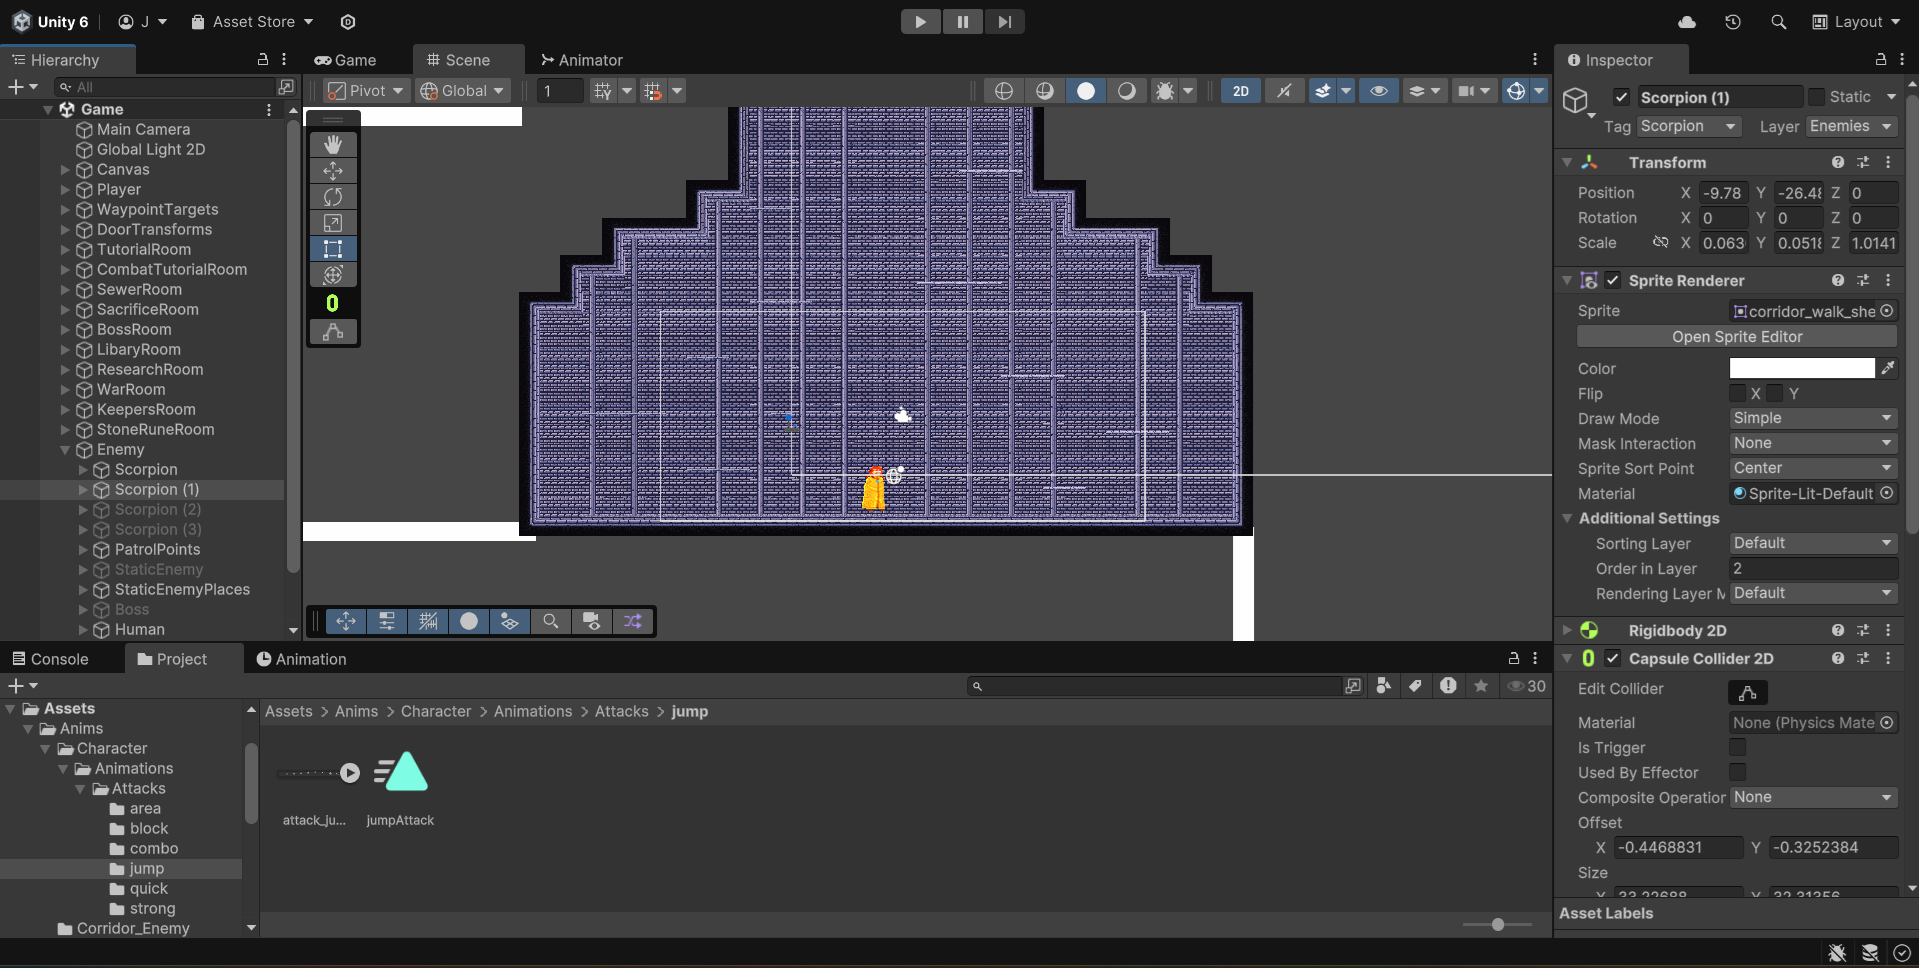
\includegraphics[width=0.9\textwidth]{UnityEditorKep.png}
	\caption{Unity Editor}
	\label{fig:unityEditor}
\end{figure}

\subsubsection{Scene View}
A Scene View az Editor egyik legfontosabb része. Itt láthatod vizuálisan,szerkesztheted a játékot. A GameObjecteket itt választhatod ki, itt módosíthatod őket. A Scene View egy interaktív ablak amely megkönnyíti a jelenetek felépítését.\cite{UnityScene}
\subsubsection{Game View}
A Game View a játék végső, futtatott állapotát mutatja. Ez a nézet a projektben elhelyezett kamerák által renderelt képet jeleníti meg.\cite{UnityGameView}

\subsubsection{Inspector}
Az Inspector ablakban található a kijelölt GameObject összes tulajdonsága,komponense. Itt lehet módosítani a kijelölt GameObject tulajdonságait, hozzáadni/eltávolítani komponenseket.\cite{UnityIspector}

\subsubsection{Hierarchy window}
Ebben az ablakban minden GameObject megjelenik a jelenetben,Ezt az ablakot lehet használni a GameObjectek rendszerezésére.\cite{UnityIspector}
\subsubsection{Project window}
Ebben az ablakban megjelenik minden fájl/mappa ami a projektben van, itt tudsz navigálni a fájlok között.\cite{UnityProject}
\subsubsection{Animator window}

\begin{figure}[h!]
	\centering
	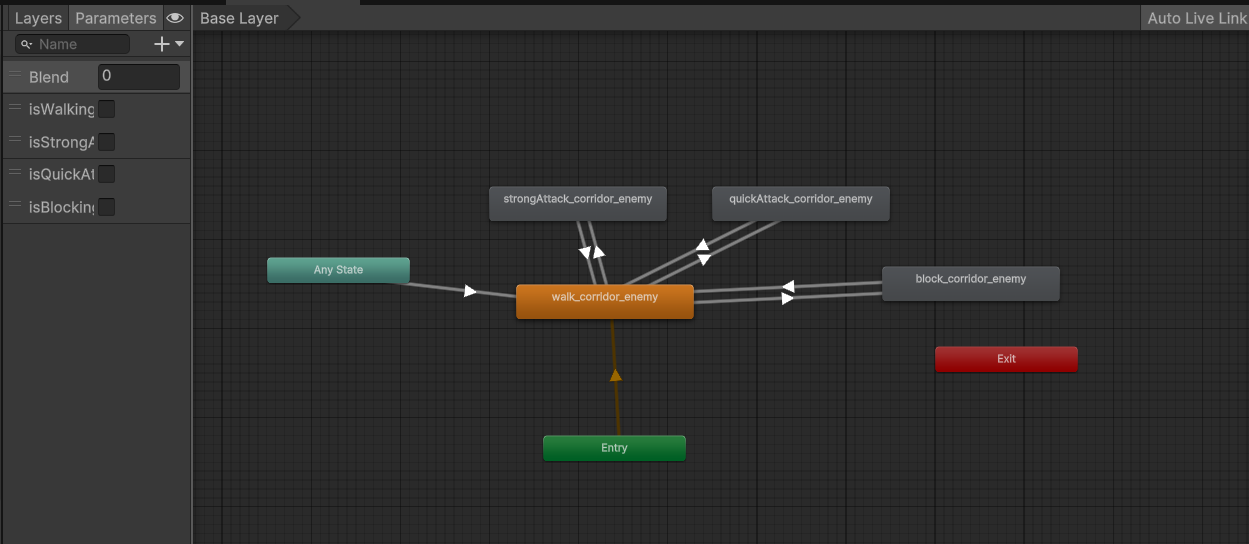
\includegraphics[width=0.9\textwidth]{UnityAnimatorKep.png}
	\caption{Unity Animator}
	\label{fig:unityAnimator}
\end{figure}
Az Animator lehetővé teszi az animációk és azok közötti átmenetek kezelését és irányítását. Általában több animációra van szükség és ezek között átmeneteket kell létrehozni amikor bizonyos játékbeli események történnek. Például ha a játékos megnyomja az SHIFT gombot akkor séta animációból átmegy futás animációba.Az átmeneteket állapot géppel kezeli az Animator.\cite{UnityAnimatorController}

\subsubsection{Animation window}
Az Animation ablakban lehet megnézni, módosítani, hozzáadni az animációkat a GameObjecteken. A GameObjecten kell lennie egy Animator komponensnek hogy a GameObject animáció látszódjanak a játékban.\cite{UnityAnimation}

\chapter{Rendszerterv}

\section{A rendszer célja}
A szakdolgozatom célja egy kétdimenziós platformer típusú videojáték fejlesztése, amelyben a játékos egy oldalsó nézetű világban irányít egy karaktert. A játék során a játékos különböző pályákon halad keresztül, miközben akadályokat küzd le, ugrásokkal manőverezik, valamint különböző típusú ellenségekkel harcol. A pályák teljesítésével a játékos fokozatosan halad előre a szinteken, egyre nehezebb kihívásokkal szembesülve.
A fejlesztés során a grafikai elemeket -- beleértve háttereket, karakter animációkat, felhasználói felület elemeket valamit az összes dizájnhoz kapcsolódó komponenst -- egy külön grafikus készítette.  A grafikus szakdolgozati munkája szorosan kapcsolódik az én projektemhez, ugyanis ő saját szakdolgozata keretében dolgozta ki és valósította meg a játék látványvilágát. Ez az együttműködés lehetővé tette, hogy a játék egységes vizuális stílusban készüljön el, amely nemcsak esztétikai szempontból emeli a színvonalat, hanem hozzájárul a játék hangulatának és egyediségének kialakításához is. A közös munka során a látványterveket és az animációkat folyamatosan egyeztettük, hogy azok minél jobban illeszkedjenek a játékmenethez és a játék által képviselt világ hangulatához.
\section{Projektterv}
A projekt célja egy kétdimenziós platformer videojáték elkészítése Unity játékmotor segítségével, amelyben a játékos harcol, ugrál, és különféle akadályokat leküzdve jut tovább a szinteken. A projekt megvalósításához két fő erőforrás állt rendelkezésre: a fejlesztő (jelen szakdolgozat készítője) és a grafikus, akik külön-külön, de összehangoltan dolgoztak a játék létrehozásán.
\subsubsection{Szerepkörök}
\begin{itemize}
	\item Fejlesztő \\A játék mechanikáinak, működésének, szintlogikájának és programkódjának megvalósítása. Felelős volt a Unity projekthez kapcsolódó összes technikai döntésért, valamint a grafikus által készített assetek integrálásáért.
	\item Grafikus \\A játékhoz szükséges összes vizuális elem – háttérképek, karakterek, animációk, UI-elemek – megtervezése és elkészítése. A grafikus saját szakdolgozata keretében dolgozott, így a vizuális tartalom elkészítése önálló projektként, de szorosan együttműködve zajlott.
\end{itemize}

\subsubsection{Felelősségek}
\begin{tabular}{|c|c|c|}
	\hline
	Név & Szerep & Felelősségek\\
	\hline
	Szakdolgozó & Fejlesztő & Játékmenet logika,programozás,hibajavítás \\
	\hline
	Grafikus & Látványtervező & Sprite-ok,animációk, UI elemek, háttérképek elkészítése \\
	\hline
\end{tabular}
A fejlesztő és a grafikus rendszeres konzultációk során hangolták össze a játékmenetet és a látványvilágot, hogy a kész játék esztétikailag is egységes élményt nyújtson.

\subsubsection{Mérföldkövek}
\begin{table}[h!]
	\centering
	\begin{tabular}{|p{4cm}|p{12cm}|}
		\hline
		\textbf{Mérföldkő} & \textbf{Leírás} \\
		\hline
		Alapjátékmechanikák elkészítve & A játékos mozgása, ugrása, ütközésérzékelés működőképes \\
		\hline
		Ellenségek implementálva & Legalább egy típusú ellenség működik, harcol a játékossal \\
		\hline
		Első játszható szint elkészítve & Egy teljes pálya bejárható, vizuális elemek nélkül \\
		\hline
		Grafikai integráció befejezve & A grafikus által készített sprite-ok, animációk beépítve a játékba \\
		\hline
		Teljes játszható verzió készen & A játék játszható állapotban van több szinttel, harccal, vizuálisokkal \\
		\hline
		Tesztelés és finomhangolás & A játék stabilan fut, főbb hibák javítva \\
		\hline
	\end{tabular}
	\caption{Fejlesztési mérföldkövek}
\end{table}
\section{Funkcionális terv}
A funkcionális terv célja a játék funkcióinak részletes technikai leírása a fejlesztő szemszögéből, a funkcionális specifikáció alapján. A terv bemutatja a rendszer szereplőit, a fő használati eseteket és azok lefutását, a határosztályokat, valamint a menürendszer és a képernyők logikai felépítését. A játék Unity játékmotorban készült, C\# programozási nyelven.

\subsection{Rendszer szereplők}
\begin{table}[h!]
	\centering
	\begin{tabular}{|p{3cm}|p{11cm}|}
		\hline
		\textbf{Szereplő} & \textbf{Leírás} \\
		\hline
		Játékos & A játék fő irányítója, aki a karakter mozgását és interakcióit végzi. \\
		\hline
		Ellenség & AI által vezérelt ellenfél, amely a játékost támadja, vagy akadályozza. \\
		\hline
		Játékrendszer & A háttérben működő logika, amely kezeli a szinteket, életerőt, stb. \\
		\hline
	\end{tabular}
	\caption{A játék szereplői és funkcióik}
\end{table}

\subsection{Rendszerhasználati esetek és lefutásaik}
\begin{enumerate}
	\item \textbf{Játék indítása} \\
	Használati eset: A játékos elindítja a játékot a főmenüből.
	
	Lefutás:
	\begin{itemize}
		\item A főmenü megjelenik.
		\item A játékos a „Start” gombra kattint.
		\item A rendszer betölti az első pályát.
	\end{itemize}
	
	\item \textbf{Mozgás és ugrás} \\
	Használati eset: A játékos a karakterrel mozog és ugrik.
	
	Lefutás:
	\begin{itemize}
		\item A játékos lenyomja a bal/jobb nyílbillentyűt vagy „A” / „D” billentyűt.
		\item A karakter ennek megfelelően mozog balra vagy jobbra.
		\item A játékos megnyomja a „W” billentyűt, a karakter ugrik.
	\end{itemize}
	
	\item \textbf{Harc ellenséggel} \\
	Használati eset: A játékos közelharcban vagy távolsági támadással ellenséget támad.
	
	Lefutás:
	\begin{itemize}
		\item A játékos lenyomja a támadás gombot.
		\item A karakter animációja lefut, a közelben lévő ellenség életereje csökken.
		\item Az ellenség visszatámadhat.
		\item Ha az életereje 0, az ellenség meghal.
	\end{itemize}
	
	\item \textbf{Szoba teljesítése} \\
	Használati eset: A játékos teljesíti a szobát.
	
	Lefutás:
	\begin{itemize}
		\item A játékos belép a szoba végét jelző trigger zónába.
		\item A rendszer betölti a következő szobát.
		\item A játékmenet folytatódik.
	\end{itemize}
\end{enumerate}
\subsection{Menühierarchiák}
\begin{itemize}
	\item \textbf{Főmenü}
	\begin{itemize}
		\item Játék indítása
		\item Beállítások
		\begin{itemize}
			\item Hang beállítások
			\item Képernyő felbontás
			\item Teljes képernyő
		\end{itemize}
		\item Kilépés
	\end{itemize}
	\item \textbf{PauseMenü}
	\begin{itemize}
		\item Folytatás
		\item Beállítások
		\begin{itemize}
			\item Hang beállítások
			\item Képernyő felbontás
			\item Teljes képernyő
		\end{itemize}
		\item Kilépés
	\end{itemize}
\end{itemize}
\section{Követelmények}
A követelmények a rendszer fejlesztése során követendő irányelvek és célok, amelyek a játék funkcionalitását és működését határozzák meg. A követelmények a fejlesztési fázis során változhatnak, de az alábbiakban szereplő követelmények képezik a rendszerterv alapját. Ezek a követelmények az elkészítendő játék megvalósítását célozzák meg, és minden fontos funkciót, teljesítendő elvárást tartalmaznak.
\subsection{Funkcionális követelmények}
\begin{itemize}
	\item[$\bullet$] Felhasználói felület \\A játékban világos információk jelenjenek meg a játékos számára, például életerő, állóképesség, objektív mutatása és egyéb információk.
	\begin{itemize}
		\item \textbf{Elvárás:}A UI-elemeknek tisztán és jól láthatóan kell elhelyezkedniük, hogy a játékos könnyen hozzáférjen a szükséges információkhoz.
	\end{itemize}
	\item[$\bullet$]Tárgyak kezelése\\A játékos a pályákon található tárgyakat összegyűjtheti, de azok használata nem szükséges a játék előrehaladásához.
	\begin{itemize}
		\item \textbf{Elvárás:} A tárgyak kezelése intuitív módon történjen, és a játékos könnyen megtalálhassa a kívánt elemeket.
	\end{itemize}
	\item[$\bullet$] Harc rendszer\\ A játékos támadása az ellenségekkel való közelharc során, valamint a távolsági támadások (pl. lövedékek).
	\begin{itemize}
		\item \textbf{Elvárás:}A harci mechanizmusoknak egyszerűnek és jól irányíthatónak kell lenniük, hogy a játékos könnyedén részt vehessen a harcokban.
	\end{itemize}
	\item[$\bullet$] Játékos mozgás\\ A játékos karakterének mozgatása a bal és jobb irányban, valamint ugrás végrehajtása a "W" billentyű lenyomásával.
	\begin{itemize}
		\item \textbf{Elvárás:} A játékos simán és folyamatosan mozoghat a pályán, ugrásai életszerűek és dinamikusak legyenek.
	\end{itemize}
\end{itemize}
\subsection{Nem funkcionális követelmények}
\begin{itemize}
	\item[$\bullet$] Teljesítmény \\ A játék futása simának kell lennie minden célszámítógépen, legalább 30 FPS (képkocka/másodperc) sebességgel.
	\begin{itemize}
		\item \textbf{Elvárás:}A játéknak gyorsan reagálnia kell, és nem szabad akadoznia még nagyobb szintű grafikai elemek vagy több ellenség jelenléte esetén sem.
	\end{itemize}
	\item[$\bullet$] Hozzáférhetőség\\ A játék kezelőfelületének könnyen használhatónak kell lennie minden játékos számára.
	\begin{itemize}
		\item \textbf{Elvárás:} felhasználói felület egyszerű, könnyen navigálható és átlátható legyen.
	\end{itemize}
	\item[$\bullet$] Kép-- és hangminőség\\A grafikáknak és a hangoknak élesnek, tisztának kell lenniük, és nem szabad akadozniuk, illetve elcsúszniuk a játékos mozgásával.
	\begin{itemize}
		\item \textbf{Elvárás:} A grafikai elemeknek és hangoknak összhangban kell lenniük a játékmenettel és a játék hangulatával.
	\end{itemize}
\end{itemize}
Ezek a követelmények képezik a fejlesztés alapját, és a jövőbeni fejlesztési fázisok során figyelembe kell venni őket a megfelelő tervezési és implementálási döntések meghozatalakor.

\section{Használt fejlesztői eszközök}
\subsection{Unity}
A játék fejlesztése a Unity játékmotor segítségével történt. A Unity a világ egyik legnépszerűbb fejlesztői környezete, amely kiemelkedő rugalmasságot biztosít a különböző típusú játékok készítésében, legyen szó 2D vagy 3D játékokról. A játékfejlesztési folyamat során a Unity biztosította az összes szükséges eszközt a játékmenet logikájának, a grafikai elemek kezelésének, az animációk és fizikai rendszerek integrálásának, valamint a felhasználói interakciók kezelésének megvalósításához. A Unity fejlesztői környezetet és komponenseit a \ref{sec:Unity}. szekcióban mutatom be.
\subsection{Github,Git}
A GitHub egy felhőalapú verziókezelő platform, amely a Git verziókezelő rendszert használva lehetővé teszi a projektek tárolását, megosztását és a fejlesztők közötti együttműködést. A Git lehetővé teszi a fájlok különböző verzióinak kezelését, míg a GitHub biztosítja a központi tárolót, ahol a fejlesztők szinkronizálhatják munkájukat.\cite{GithubAndGit}
\subsection{Trello}
A Trello egy vizuális projektmenedzsment eszköz, amely segít a feladatok és projektek rendszerezésében. Kártyák és táblák segítségével a csapatok könnyen nyomon követhetik a munka előrehaladását. A felhasználók különböző kategóriákba rendezhetik feladataikat, hozzárendelhetnek határidőket, és megoszthatják a munkát másokkal.\cite{Trello}


\chapter{Saját projekt fejlesztése}
\section{A platformer játék bemutatása}
A szakdolgozat keretében egy 2D-s platformer játékot fejlesztettem Unity játékmotor segítségével. A játék lényege, hogy a játékos különböző szinteken, úgynevezett „szobákon” halad keresztül, miközben különféle ellenségekkel harcol, akadályokat kerül ki, és a célpont (waypoint) irányába mozog.A játékos számára a fő kihívást az ellenségek legyőzése, illetve a szintek közötti előrehaladás során szükséges platformugrások jelentik.

A játék vizuális elemeit – háttér, karakterek, animációk, UI – egy külön grafikus tervezte és készítette, aki szintén a szakdolgozatát ebben a témában írta. A látványvilág egyedi, pixel art stílusú, így kifejezetten karakteres megjelenést biztosít a játéknak.
\subsection{A játékos karakter}
A játékos egy karaktert irányít, aki képes:
\begin{itemize}
	\item[$\bullet$] balra és jobbra mozogni
	\item[$\bullet$] ugrani
	\item[$\bullet$] különféle támadásokat végrehajtani mint például a gyors, erős területi, ugró támadás.
\end{itemize}
A karakter rendelkezik életerővel, amely csökken, ha az ellenségek megsebesítik. Ha az életerő eléri a nullát, a karakter meghal, és a játék az utolsó checkpoint-tól indul újra.A karakter rendelkezik még állóképességgel is , amely csökken, ha fut vagy erős,területi támadást használ.
A karakter mozgása és animációi pontosan követik a játékos parancsait, ezzel biztosítva a gördülékeny játékmenetet.
\subsection{Ellenségek}

A játékban többféle ellenség jelenik meg, amelyek különböző támadási és mozgási mintákkal rendelkeznek. Ezeket hardcode-olt AI vezérli, és a játékos közelébe érve aktívvá válnak.
\begin{itemize}
	\item Skorpió
	\begin{itemize}
		\item \textbf{Mozgás}:Alapvetően, ha a játékos nincs az ellenség üldözési távolságában, az ellenség két kijelölt pont között oda-vissza mozog.
		\item \textbf{Viselkedés}:Amikor a játékos belép az ellenség üldözési távolságába, az skorpió elindul felé, és ha elég közel ér hozzá, támadásba lendül és elkezdi támadni a játékost.
		\item \textbf{Támadásai}:A skorpió támadásai közelharciak:
		\begin{itemize}
			\item Gyors támadás: A gyors támadás egy gyors, alacsonyabb sebzéssel járó támadás, amely lehetőséget ad az ellenség számára, hogy gyorsan reagáljon a játékos mozgására. A gyors támadások kisebb sebzést okoznak, de sokkal gyorsabban végrehajthatók, lehetővé téve az ellenség számára, hogy folyamatos nyomást gyakoroljon a játékosra. 
			\item Erős támadás: Az erős támadás egy lassabb, de erősebb támadás, amely nagyobb sebzést okoz a játékosnak. Az ellenség a támadás során jobban felkészül, hogy egy erőteljes ütéssel sújtsa a játékost. Az erős támadás lassabb mint a gyors, így a játékosnak van lehetősége elkerülni vagy blokkolni, de sikeres eltalálás esetén komolyabb sebzést eredményez.
		\end{itemize}
		Ezen kívül a skorpió képes blokkolni a játékos támadásait, miközben a saját támadásai között váltogat.
	\end{itemize}
	\item Csatornai Ellenség
	\begin{itemize}
		\item \textbf{Mozgás}:Alapvetően ez az ellenség statikus, egy helyen áll, és csak akkor mozdul el, ha az életereje 20 alá csökken.
		\item \textbf{Viselkedés}:Az ellenség viselkedése a saját életerejétől és a játékos helyzetétől függ:
		\begin{itemize}
			\item Ha a játékos a szobában tartózkodik, az ellenség folyamatosan támadja őt.
			\item Ha a játékos 3 lövedékét blokkolja, utána egy ideig nem tud támadni. Így a játékos egy rövid szünetet kap, hogy reagálhasson.
			\item Amikor a saját életereje 20 alá csökken,akkor elmozdul a helyéről, hogy új pozíciót vegyen fel.Ilyenkor az életereje vissza megy a max életerejére. Ezt a műveletet legfeljebb kétszer ismételheti meg.
			\item Miután kétszer elmozdult, a játékos szabadon legyőzheti.
			
		\end{itemize}
		\item \textbf{Támadásai}: A támadásai távol harciak:
		\begin{itemize}
			\item Egy lövedéket lő ki a játékos felé. Ha ez a lövedék egy akadálynak ütközik, például egy falnak vagy a játékos pajzsának ,akkor a lövedék megsemmisül, és nem okoz sebzést.
			\item Ha a lövedék eléri a játékost, akkor sebzést okoz.
		\end{itemize}
		
	\end{itemize}
	\item Ember
	\begin{itemize}
		\item \textbf{Mozgás}:Amikor a játékos nem tartózkodik a szobában, az ellenség inaktívvá válik, és csak egy idle animációt hajt végre. Ebben az állapotban nem reagál semmilyen eseményre, és nem végez támadásokat vagy egyéb akciókat, amíg a játékos vissza nem tér a szobába.
		\item \textbf{Viselkedés}:Amikor a játékos a szobában tartózkodik, az ellenség automatikusan elindul felé. Amint elég közel kerül a játékoshoz, megkezdi a támadást. Ez a viselkedés biztosítja, hogy az ellenség mindig aktívan reagáljon a játékos jelenlétére, és ne maradjon inaktív, ha a játékos a közelben van.
		\item \textbf{Támadásai}:Az ember támadásai közelharciak:
		\begin{itemize}
			\item gyors támadás
			\item Erős támadás
			\item Roham támadás: Amikor a játékos belép az ellenség rohamkörébe, az ellenség aktiválhatja a roham támadást, amely során hirtelen nekiront a játékosnak, és gyorsan elér egy közvetlen támadást. Ez a mozdulat lehetővé teszi az ellenség számára, hogy gyorsan reagáljon a játékos jelenlétére.
		\end{itemize}
		Ezen kívül az ember ellenség képes blokkolni a játékos támadásait, miközben a saját támadásai között váltogat.
	\end{itemize}
	\item Boss
	\begin{itemize}
		\item \textbf{Mozgás}:Amikor a játékos nem tartózkodik a szobában, az ellenség inaktívvá válik, és csak egy idle animációt hajt végre. Ebben az állapotban nem reagál semmilyen eseményre, és nem végez támadásokat vagy egyéb akciókat, amíg a játékos vissza nem tér a szobába.
		\item \textbf{Viselkedés}:Amikor a játékos a szobában tartózkodik, az ellenség automatikusan elindul felé. Amint elég közel kerül a játékoshoz, megkezdi a támadást. Ez a viselkedés biztosítja, hogy az ellenség mindig aktívan reagáljon a játékos jelenlétére, és ne maradjon inaktív, ha a játékos a közelben van.
		\item \textbf{Támadásai}:A támadásai neki is közelharciak, viszont az életerejétől függően 2 fázisra vannak osztva a támadások.
		\begin{itemize}
			\item Első fázis: Amikor az életereje 150 és 300 azaz a max életereje között van:
			\begin{itemize}
				\item Erős támadás
				\item Területi támadás:A területi támadás olyan támadást jelent, amely egy nagy területen ad sebzést. Az ellenség egy szélesebb hatótávolságú támadást hajt végre,és ha a játékos benne van ebben a hatótávban akkor sebzést kap.
			\end{itemize}
			\item Második fázis:
			\begin{itemize}
				\item Roham támadás
				\item Gyors támadás
			\end{itemize}
			\item fázistól függetlenül tudja a játékos támadásait kivédeni, miközben a saját támadásai között váltogat.
		\end{itemize}
	\end{itemize}
\end{itemize}

\subsection{Pályarészek közötti átjárás}
A pályá úgy van kialakítva, hogy külön „szobákra” van osztva. Minden szoba egy különálló rész a játéktérben, és a játékos egy átjárón keresztül tud átjutni a következőbe.

A szobák közti átjárás logikája:
\begin{itemize}
	\item[$\bullet$] A játékos eléri a kijáratot a szobában.
	\item[$\bullet$] Egy „trigger” érzékeli a belépést. Itt két dolog történhet:\\
	\begin{itemize}
		\item Ha a játékos teljesítette a szobában lévő feladatot akkor át engedheti
		\item Ha még nem teljesítette akkor viszont ki ír a képernyőre egy üzenetet, ami tartalmazza a feladatot.
	\end{itemize}
	\item[$\bullet$] A rendszer átrakja a karaktert a következő szobába miközben egy rövid ideig elsötétül a képernyő.
	\item[$\bullet$] A játékos pozíciója automatikusan beállításra kerül az új szobán belüli kezdőpontra.
\end{itemize}
Ha a játékos szeretné vissza is tud menni egy előző szobába és onnan már egyből tud tovább menni a következő szobába.

\subsection{Waypoint mutató}
A játékos tájékozódását egy waypoint mutató segíti, amely mindig az aktuális cél irányába mutat:
\begin{itemize}
	\item Ha a cél (pl. következő kijárat, fontos tárgy, vagy ellenség) nem látszik a képernyőn, a waypoint ikon a képernyő szélén jelenik meg, és az irányt mutatja.
	\item Amennyiben a játékos a szoba aktuális célpontjának közelébe kerül, a mutató automatikusan eltűnik. A cél teljesítése után a mutató ismét megjelenik, és a következő cél irányába kezd el jelezni.
	\item Ezzel a megoldással a játékos nem téved el, és a játék élménye áramvonalasabbá válik.
\end{itemize}
Ezzel a modullal biztosítottuk, hogy a játékos ne akadhasson el a pályán, lehetővé téve a zökkenőmentes előrehaladást.

\section{Játékmechanikák és algoritmusok}
\subsection{Mozgás és irányítás}
A játékos mozgása a 2D-s fizikai motor segítségével lett implementálva, amely biztosítja a gravitációs hatásokat, valamint az ütközéseket és a platformok közötti interakciókat. A játékos irányítása az Input System-en keresztül történik, amely lehetővé teszi a billentyűzet és az egér használatát.
\subsubsection{Ellenségek Mozgása}
A játékban alkalmazott ellenségek AI-ja hardcode-olt (kézzel kódolt), amely az ellenség viselkedését és reakcióit előre meghatározott logikák alapján irányítja. Az AI működését statikus algoritmusok és feltételek szabályozzák, amelyek a játékos jelenlétére és a játékhelyzetekre reagálnak.
\subsubsection{Csatornai ellenség}
A csatornai ellenségnek az AI-ja csak akkor mozgatja az ellenséget ha az életereje 20 alá csökken, mint egy védelemi mechanizmusként. Itt a kódban meghatározott helyek tömbjében mozog, ha eléri a tömb végét akkor már nem tud helyet váltani és ekkor lehet legyőzni.
\subsubsection{Skorpió ellenség}
Az ellenség mozgása előre meghatározott pályákon zajlik. A mozgás logikája a játéktér egyes meghatározott pontjaira (waypoint) irányítja az ellenséget, amelyeket a fejlesztés során statikusan kódoltam. Az AI folyamatosan ezek között a pontok között mozog, és egy egyszerű irányítást követ, amely nem alkalmaz semmiféle dinamikus döntéshozatalt vagy alkalmazkodást.
A skorpió AI figyeli, hogy van-e alatta talaj, hogy biztosan ne essen le a pályáról. Ha nem érzékel talajt, a skorpió automatikusan megfordul, és a másik irányban lévő waypoint-hoz kezd el mozogni. Ez a viselkedés segít abban, hogy az ellenség ne menjen le a szoba legaljára amikor a játékos a szobában tartózkodik, és folyamatosan a kijelölt helyén maradjon, miközben a játékost várja.
Minden másik ellenség csak akkor kezdi el a mozgást ha a játékos beért az üldözési távolságába.
\subsection{Támadások}
A játékban az ellenség és a játékos támadásainak sebzésrendszere a következő módon van megvalósítva: minden támadásnak van egy meghatározott pontja a játékos vagy az ellenség előtt, amely körül a támadás sebzést ad. Ez a kör a támadások hatókörét reprezentálja, és minden támadás során az adott körben lévő célpontok, például a játékos, sebzést kapnak. A támadások hatóköre és a sebzés nagysága az egyes támadások típusaitól függően változhat, és a játékos vagy az ellenség helyzete alapján kerül kiszámításra.

Kivételt képez azonban a csatornai ellenség támadása, mivel az ő támadása nem a megszokott módon működik. A csatornai ellenség egy lövedéket instanciál a támadási pontján, amely a játékos felé halad. A lövedék fizikai tulajdonságait és működését a hozzá tartozó Collider komponens irányítja. A lövedék esetében a sebzés akkor kerül kiosztásra, ha a lövedék eltalálja a játékost, és a Collider ütközik a játékos Colliderével. A lövedék akkor sem okoz sebzést, ha valamilyen akadályba ütközik, vagy ha a játékos blokkolja azt, ekkor a lövedéket törölni kell, hogy az ne okozzon további problémát a játékmenetben.
\subsection{Pályarészek közti átjárás logikája}
A játékban, amikor a játékos eléri az ajtót, a rendszer automatikusan ellenőrzi, hogy a játékos teljesítette-e a szoba célját. Ha a cél nem teljesült, a rendszer egy üzenetet jelenít meg, amely tartalmazza a szoba célját, tájékoztatva a játékost arról, hogy még nem érte el a szükséges feltételeket a továbbjutáshoz.

Abban az esetben, ha a játékos sikeresen teljesítette a szoba célját, a rendszer egy „Inspect” feliratot jelenít meg az ajtó mellett, jelezve, hogy a játékos interakcióba léphet az ajtóval. Ekkor, ha a játékos az E billentyűt lenyomja, a rendszer átvált a következő szobára, lehetővé téve a továbbhaladást.

A játékban az ajtók előtt Collider2D komponensek találhatóak, amelyek trigger-re vannak állítva. Ez azt jelenti, hogy az ajtók területére lépve a rendszer automatikusan érzékeli a játékos jelenlétét. Az ellenőrzés csak akkor kezdődik el, amikor a játékos belelép a trigger zónába. A rendszer a játékos címkéjét (tag) keresi a GameObject-en, hogy megbizonyosodjon arról, hogy valóban a játékos lépett a területre, és ne aktiválódjon más objektumoknál a trigger.
Ez a megoldás biztosítja, hogy az ajtó előtt található collider csak akkor aktiválódjon, ha valóban a játékos lép be a területére, így elkerülhető, hogy más objektumok, például ellenségek vagy statikus elemek is véletlenül aktiválják a továbbjutási mechanizmust.
\subsubsection{Waypoint mutató}
A waypoint a játékban egy kis ikon, amely a Canvas-ban jelenik meg, és a kód irányítja, hogy éppen melyik irányba mutasson. Amikor a játékos elég közel ér a célhoz, a waypoint automatikusan eltűnik. Az irányítás és a célpontok közötti váltás a setWaypointTarget metódus segítségével történik, amelyet a kódban használtam. Ezt a metódust alkalmazom a Collider trigger enter eseményeknél, valamint a kontroller kódokban, hogy dinamikusan frissítsem a waypoint célpontját, amikor a játékos elér egy új szobát vagy új célt.



\chapter{Tesztelés}
A tesztelés a szoftverfejlesztés egyik legfontosabb és elengedhetetlen lépése, amely lehetővé teszi a hibák korai felismerését és kijavítását. A tesztelés során a fejlesztők és tesztelők különböző módszerekkel próbálják reprodukálni a felhasználói interakciókat, ellenőrizve, hogy a rendszer megfelelően reagál-e minden lehetséges helyzetben. A hibák észlelése és javítása nélkülözhetetlen, mivel bármilyen figyelmen kívül hagyott probléma komoly hátrányt okozhat a játék működésében, élményében és teljesítményében.

Ha a tesztelést kihagyják a fejlesztési folyamatból, akkor sokkal nehezebb azonosítani azokat a rejtett hibákat, amelyek esetleg csak bizonyos körülmények között vagy a játékosok különböző interakcióival lépnek fel. 
Én két féle tesztelési módot alkalmaztam a projektben: Playtest--et ahol körültekintően kipróbáltam minden lehetséges dolgot, itt barátaim is besegítettek a hibák keresésében. Alkalmaztam a Unity--n belül Unit testeket amit a unity Test Framework moduljával csinálta.
\section{Playtest}
\section*{Unit teszt}
\chapter*{Összegzés}
\addcontentsline{toc}{chapter}{Összegzés}
A projekt célja egy összetett játékmechanikai rendszer megvalósítása volt, amely magában foglalja a felhasználói felületet, a tárgyak kezelését, a harcrendszert, valamint a játékos mozgásának logikáját és grafikáját. Az alábbiakban összefoglalom a megvalósított rendszerek fejlesztési folyamatát és azok működését.

A felhasználói felület (UI) logikájának megvalósítása az egyik legfontosabb lépés volt a projekt során. Az UI célja, hogy a játékos számára világos és áttekinthető módon biztosítsa az összes szükséges információt, például az életpontokat, az inventory tartalmát, valamint az aktuális küldetést vagy játékmeneti státuszt. A felhasználói felület egyszerű, de hatékony kezelése alapvetően javítja a játékélményt, mivel a játékos könnyen hozzáférhet minden fontos adatponthoz anélkül, hogy a játékmenetet megszakítaná.

A tárgyak kezelése szintén kulcsfontosságú volt a projektben, mivel az inventory rendszer lehetővé teszi a játékos számára, hogy különböző tárgyakat és egyéb fontos itemeket gyűjtsön. A rendszer implementálása során biztosítottuk, hogy a játékos könnyedén hozzáférhessen a tárgyakhoz, azok használata pedig logikusan és gördülékenyen történjen.

A harcrendszer megvalósítása két fő összetevőből állt: a harc logikájának és annak grafikájának a megtervezéséből. A harci mechanizmus lényege, hogy lehetővé tegye a játékos számára az ellenségekkel való interakciót különböző támadási és védekezési módokon keresztül. A harcrendszer logikája biztosítja, hogy a harc dinamikus és szórakoztató legyen, miközben a játékos választhat a különböző támadások közül. A harc grafikájának implementálása a támadások, védekezések és a különböző effektusok vizuális megjelenítésére irányult, így a harc nemcsak logikai, hanem vizuális élményt is biztosít a játékos számára.

A játékos mozgásának logikája és grafikája az egyik legfontosabb eleme volt a projektnek. A mozgás rendszerének célja, hogy a játékos képes legyen dinamikusan navigálni a játék világában, miközben a fizikai törvények figyelembevételével történik a mozgás. A mozgás logikájának megtervezése során különös figyelmet fordítottam a gyorsaságra, az irányításra és az interakciókra. A mozgás grafikai megjelenítése biztosítja, hogy a játékos minden irányba gördülékenyen és élethűen mozogjon a környezetben, miközben a karakter animációi megfelelnek a mozgás fizikai törvényeinek.

\section{Bővítési terv}
A projekt következő bővítési fázisa a játék vizuális és mechanikai rendszerének továbbfejlesztésére irányul, különös figyelmet fordítva az item dizájnok, a grafikus UI dizájnok és a dinamikusan viselkedő ellenségek megvalósítására. Ezen elemek hozzáadásával a játék nemcsak hogy vizuálisan gazdagabbá válik, hanem a játékmenet interaktivitása és a kihívások is fokozódnak.
\chapter*{Ábrák jegyzéke}
\addcontentsline{toc}{chapter}{Ábrák jegyzéke}
\begin{center}
	\ref{fig:unityEditor}. ábra --saját ábra.\\
	\ref{fig:unityAnimator}. ábra--saját ábra.
\end{center}

\chapter*{Irodalomjegyzék}
\begin{thebibliography}{2}
\addcontentsline{toc}{chapter}{\bibname}
\bibitem{GDScript}
\textsc{Godot Engine}: \emph{GDScript}, elérhető:
\url{https://docs.godotengine.org/en/stable/tutorials/scripting/gdscript/gdscript_basics.html} [Letöltve: 2025-04-10]
\bibitem{Godot1.0}
\textsc{Godot Engine}: \emph{Version 1.0}, elérhető:
\url{https://godotengine.org/article/godot-engine-reaches-1-0/} [Letöltve: 2025-04-10]\\
\bibitem{Godot2.0}
\textsc{Godot Engine}: \emph{Version 2.0}, elérhető:
\url{https://godotengine.org/article/godot-engine-reaches-2-0-stable/} [Letöltve: 2025-04-10]\\
\bibitem{Godot3.0}
\textsc{Godot Engine}: \emph{Version 3.0}, elérhető:
\url{https://godotengine.org/article/godot-3-0-released} [Letöltve: 2025-04-10]\\
\bibitem{Godot4.0}
\textsc{Godot Engine}: \emph{Version 4.0}, elérhető:
\url{https://godotengine.org/article/godot-4-0-sets-sail} [Letöltve: 2025-04-10]\\
\bibitem{GodotLicenc}
\textsc{Godot Engine}: \emph{Licences}, elérhető:
\url{https://docs.godotengine.org/en/stable/about/complying_with_licenses.html} [Letöltve: 2025-04-10]\\

\bibitem{UnrealBlueprint}
\textsc{Unreal Engine}: \emph{Blueprint}, elérhető:
\url{https://dev.epicgames.com/documentation/en-us/unreal-engine/coding-in-unreal-engine-blueprint-vs.-cplusplus} [Letöltve: 2025-04-10]\\
\bibitem{UnrealBlueprintClasses}
\textsc{Unreal Engine}: \emph{Blueprint classes}, elérhető:
\url{https://dev.epicgames.com/documentation/en-us/unreal-engine/overview-of-blueprints-visual-scripting-in-unreal-engine} [Letöltve: 2025-04-10]\\
\bibitem{Unreal4.27}
\textsc{Unreal Engine}: \emph{Version 4.27}, elérhető:
\url{https://dev.epicgames.com/documentation/en-us/unreal-engine/unreal-engine-4.27-release-notes?application_version=4.27} [Letöltve: 2025-04-10]\\
\bibitem{Unreal5.0}
\textsc{Unreal Engine}: \emph{Version 5.0}, elérhető:
\url{https://dev.epicgames.com/documentation/en-us/unreal-engine/unreal-engine-5.0-release-notes?application_version=5.0} [Letöltve: 2025-04-10]\\
\bibitem{Unreal5.3}
\textsc{Unreal Engine}: \emph{Version 5.3}, elérhető:
\url{https://dev.epicgames.com/documentation/en-us/unreal-engine/unreal-engine-5.3-release-notes?application_version=5.3} [Letöltve: 2025-04-10]\\
\bibitem{Unreal5.5}
\textsc{Unreal Engine}: \emph{Version 5.5}, elérhető:
\url{https://www.unrealengine.com/en-US/blog/unreal-engine-5-5-is-now-available} [Letöltve: 2025-04-10]\\
\bibitem{UnrealStrengths}
\textsc{Unreal Engine}: \emph{Features}, elérhető:
\url{https://www.unrealengine.com/en-US/features} [Letöltve: 2025-04-10]\\
\bibitem{UnrealLicences}
\textsc{Unreal Engine}: \emph{Licences},elérhető
\url{https://www.unrealengine.com/en-US/license} [Letöltve: 2025-04-10]\\

\bibitem{Csharp}
\textsc{Microsoft}: \emph{C\# language documentation}, elérhető:
\url{https://learn.microsoft.com/en-us/dotnet/csharp/} [Letöltve: 2025-04-10]\\
\bibitem{Unity4.0}
\textsc{Unity}: \emph{Version 4.0}, elérhető:
\url{https://unity.com/news/unity-4-0-launches} [Letöltve: 2025-04-10]\\
\bibitem{Unity5.0}
\textsc{Unity}: \emph{Version 5.0}, elérhető:
\url{https://unity.com/news/unity-5-here} [Letöltve: 2025-04-10]\\
\bibitem{Unity6}
\textsc{Unity}: \emph{Version 6}, elérhető:
\url{https://unity.com/releases/unity-6-releases} [Letöltve: 2025-04-10]
\bibitem{UnityLicences}
\textsc{Unity}: \emph{Licences}, elérhető:
\url{https://unity.com/products/compare-plans} [Letöltve: 2025-04-10]
\bibitem{UnityScene}
\textsc{UnityScene}: \emph{Creating scenes}, elérhető:
\url{https://docs.unity3d.com/Manual/CreatingScenes.html} [Letöltve: 2025-04-10]
\bibitem{UnityGameObject}
\textsc{UnityGameObject}: \emph{GameObject}, elérhető:
\url{https://docs.unity3d.com/6000.0/Documentation/Manual/class-GameObject.html} [Letöltve: 2025-04-10]
https://docs.unity3d.com/Manual/Components.html
\bibitem{UnityComponents}
\textsc{Unity}: \emph{Introduction to components}, elérhető:
\url{https://docs.unity3d.com/Manual/Components.html} [Letöltve: 2025-04-10]
\bibitem{UnityTransform}
\textsc{Unity}: \emph{Transforms}, elérhető:
\url{https://docs.unity3d.com/Manual/class-Transform.html} [Letöltve: 2025-04-10]
\bibitem{UnityCollider}
\textsc{Unity}: \emph{Collider2D}, elérhető:
\url{https://docs.unity3d.com/Manual/2d-physics/collider/collider-2d-landing.html} [Letöltve: 2025-04-10]
\bibitem{UnityRigidBody}
\textsc{Unity}: \emph{Introduction to RigidBody 2D}, elérhető:
\url{https://docs.unity3d.com/Manual/2d-physics/rigidbody/introduction-to-rigidbody-2d.html} [Letöltve: 2025-04-10]

\bibitem{UnitySpriteRenderer}
\textsc{Unity}: \emph{Sprite renderer}, elérhető:
\url{https://docs.unity3d.com/Manual/sprite/renderer/renderer-landing.html} [Letöltve: 2025-04-10]
\bibitem{UnityScript}
\textsc{Unity}: \emph{Introduction to scripting}, elérhető:
\url{https://docs.unity3d.com/Manual/intro-to-scripting.html} [Letöltve: 2025-04-10]
\bibitem{UnityLight}
\textsc{Unity}: \emph{Lighting}, elérhető:
\url{https://docs.unity3d.com/Manual/Lighting.html} [Letöltve: 2025-04-10]\\
\bibitem{UnityPrefabs}
\textsc{Unity}: \emph{Prefabs}, elérhető:
\url{https://docs.unity3d.com/Manual/Prefabs.html} [Letöltve: 2025-04-10]\\
\bibitem{UnityScene}
\textsc{Unity}: \emph{Using the scene view}, elérhető:
\url{https://docs.unity3d.com/Manual/UsingTheSceneView.html} [Letöltve: 2025-04-10]\\
\bibitem{UnityGameView}
\textsc{Unity}: \emph{Game view}, elérhető:
\url{https://docs.unity3d.com/Manual/GameView.html} [Letöltve: 2025-04-10]\\
\bibitem{UnityAnimatorController}
\textsc{Unity}: \emph{Animator Controller window}, elérhető:
\url{https://docs.unity3d.com/Manual/class-AnimatorController.html} [Letöltve: 2025-04-10]\\
\bibitem{UnityIspector}
\textsc{Unity}: \emph{Inspector window}, elérhető:
\url{https://docs.unity3d.com/Manual/UsingTheInspector.html} [Letöltve: 2025-04-10]
\bibitem{UnityHierarchy}
\textsc{Unity}: \emph{Hierarchy window}, elérhető:
\url{https://docs.unity3d.com/Manual/Hierarchy.html} [Letöltve: 2025-04-10]\\
\bibitem{UnityProject}
\textsc{Unity}: \emph{Project view}, elérhető:
\url{https://docs.unity3d.com/Manual/ProjectView.html} [Letöltve: 2025-04-10]\\
\bibitem{UnityAnimation}
\textsc{Unity}: \emph{Animation window}, elérhető:
\url{https://docs.unity3d.com/Manual/AnimationEditorGuide.html} [Letöltve: 2025-04-10]\\
\bibitem{UnityAnimatorComponent}
\textsc{Unity}: \emph{Animator component}, elérhető:
\url{https://docs.unity3d.com/Manual/class-Animator.html} [Letöltve: 2025-04-10]\\

\bibitem{GithubAndGit}
\textsc{Github}: \emph{About GitHub and Git}, elérhető:
\url{https://docs.github.com/en/get-started/start-your-journey/about-github-and-git} [Letöltve: 2025-04-10]\\
\bibitem{Trello}
\textsc{Atlassian}: \emph{Trello}, elérhető:
\url{https://trello.com/guide} [Letöltve: 2025-04-10]\\
\end{thebibliography}

% Aláírt, szkennelt nyilatkozat beillesztése a szakdolgozat végére
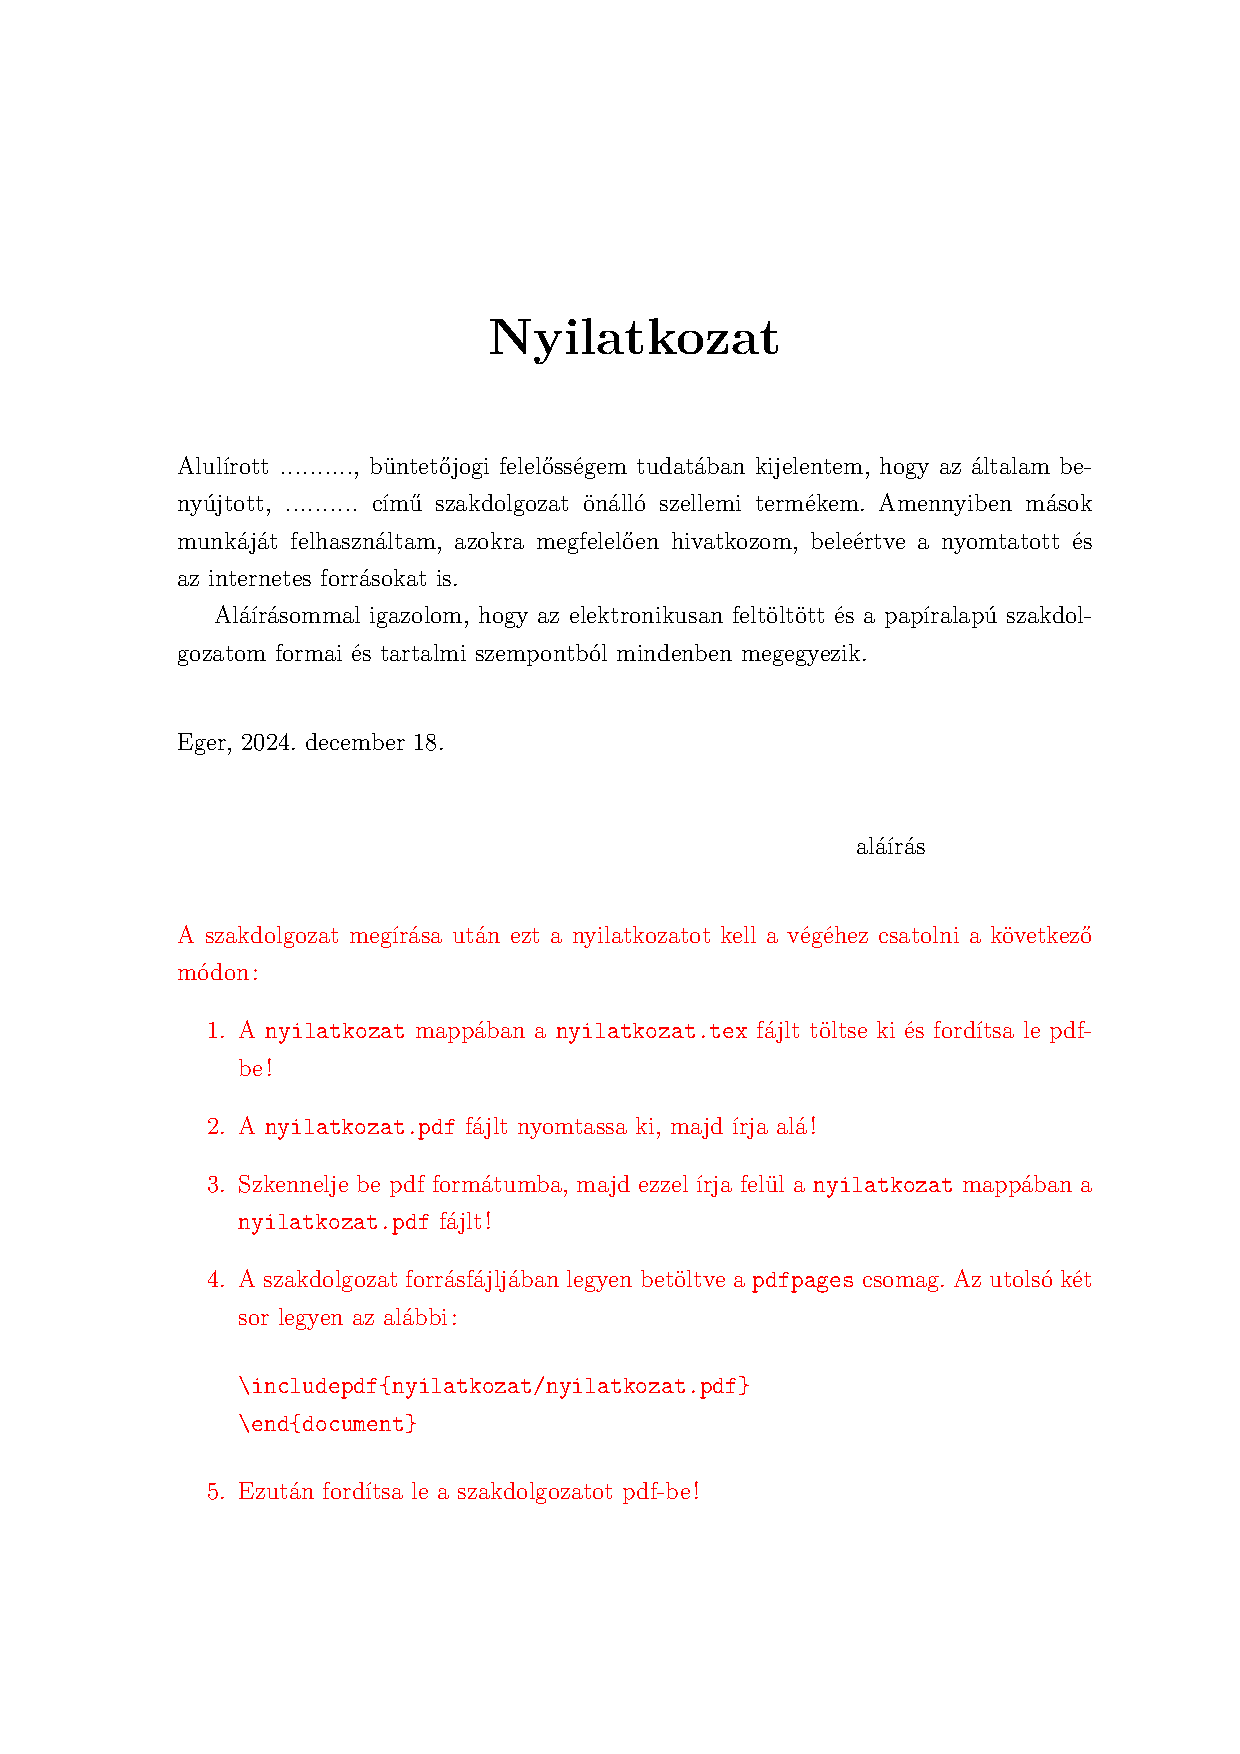
\includepdf{nyilatkozat/nyilatkozat.pdf}
\end{document}